
\chapter{Introduction\label{chpt:introduction}}

This thesis details the development of an original numerical toolkit
for physical chemists and structural biologists based on the molecular
density functional theory (\acs{MDFT}), which makes it possible to
predict the solvation properties of arbitrary molecular objects in
arbitrary molecular solvents (mainly water) efficiently and with microscopic
accuracy. In this introduction, we will explore the reasoning it explains
behind why so much research is done upon the nature of solvation,
and what are the present computing trends in solvation simulations.


\section{Simulation of solvent effects}

Solvation is a fundamental phenomenon in chemistry. The chemical behavior
of numerous systems strongly depends on the nature of solvency, including
popular issues like metal-organic reacting centers \citep{Mn-oxo,PCET},
or pharmaceutical etudes \citep{drug_1_Perlovich,drug_2_Perlovich,drug_3}.
The solvation properties required by scientific studies are highly
variable, such as the Gibbs free energy of solvation, solubility,
partition coefficient, saturated vapor pressure, pH value, the 3D
solvation structure, etc. Overall, the interest in these solvation
properties reaches into many domains such as chemistry, biochemistry,
pharmaceuticals, medicine, and environmental and agrochemical industries
\textcolor{red}{{[}ref{]}}. Unlike the well-studied quantum mechanics
(\acs{QM}) for chemical interaction and macroscopic finite element
model for physical processes, the theories of solvation are quite
variable and still under development, owing to the ambiguous compromise
between accuracy and computing cost. In a word, the studies in this
domain are quite vibrant.

\begin{figure}[h]
\centering{}\textcolor{red}{}%
\begin{minipage}[t]{1\textwidth}%
\begin{center}
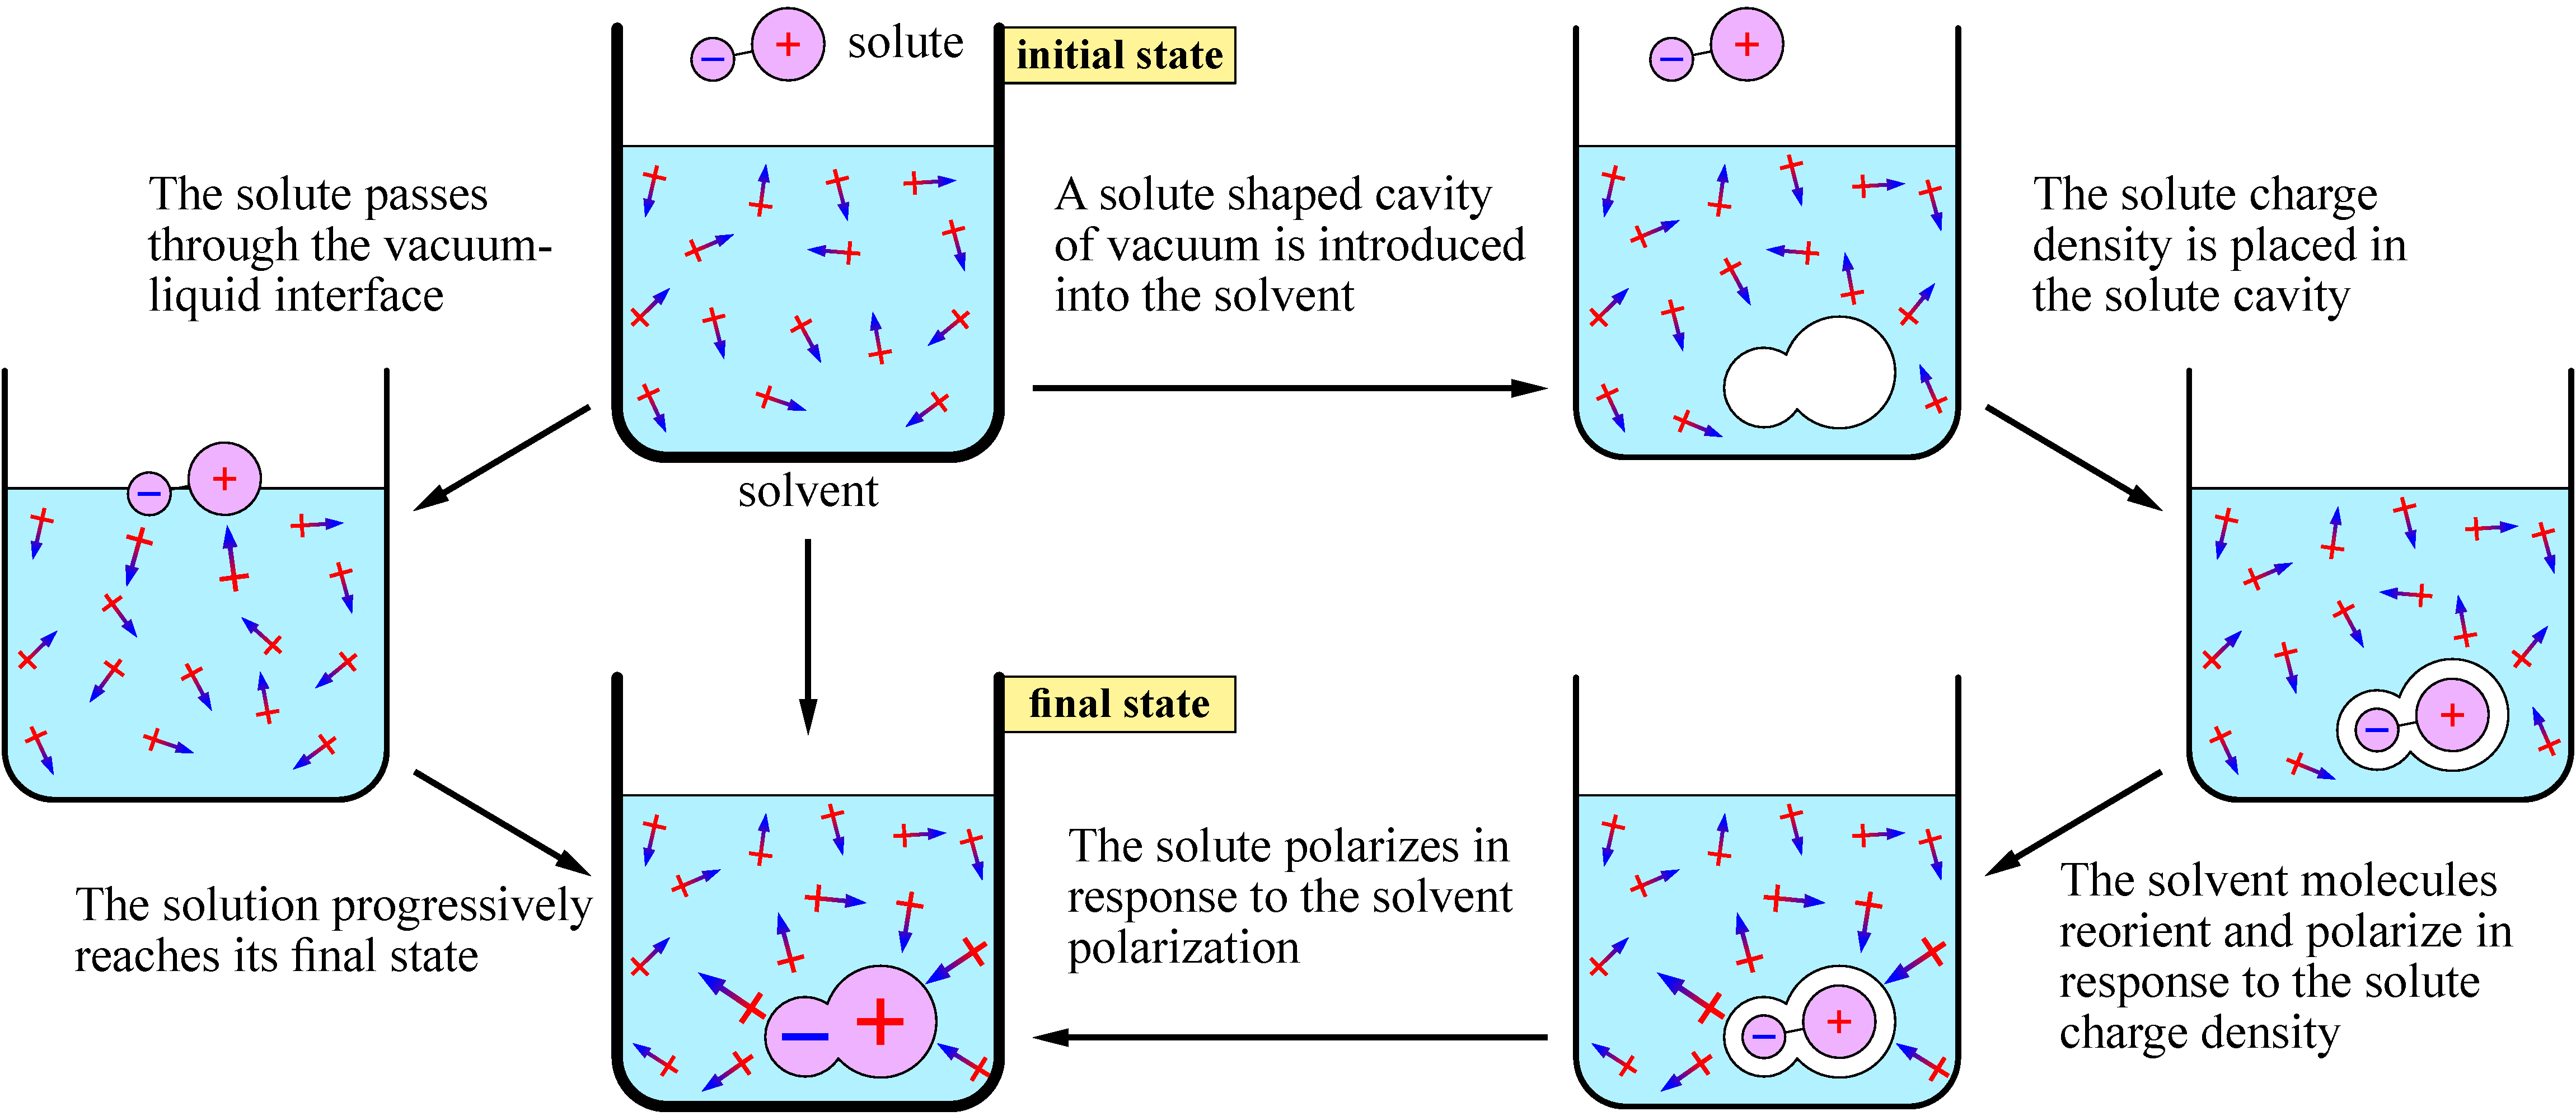
\includegraphics[width=1\columnwidth]{_figure/solvation}\caption[The solvation process]{The solvation process.\label{fig:Process-of-solvation} A thermodynamic
system, whose properties only depend on the initial and final states,
can go through different paths. The physical process of solvation
(left path) takes the solute from vacuum into bulk solvent, progressively
passing through the vacuum-liquid interface. Theoretically, the solvation
energy is defined as the energy consumed in such a process. In theoretical
studies, the process can be decomposed to some artificial unphysical
process (right path), involving the growth of an uncharged solute-sized
cavity within the bulk solvent, the transfer of the solute charge
distribution from vacuum into cavity, and the interaction between
the solute and solvent.}

\par\end{center}%
\end{minipage}
\end{figure}


To change a phenomenon to a model, we must first understand its process.
Solvation is defined as the process of moving a molecule from the
gas phase (or vacuum) to a condensed phase (figure \ref{fig:Process-of-solvation}),
which builds a stabilizing interaction with the solute (or solute
moiety like protein residues, interfaces, etc.). Such interactions
are mostly classical, involving electrostatic and van der Waals forces,
with additional more specific chemical effects such as hydrogen bond
formation, and quantic effects for some small solvents whose vibrational
or rotational energy states are at the same magnitude as $k_{\mathrm{B}}T$,
etc. \citep{Gray-Gubbins,iupac}.

As not all kinds of interactions are important in applications, different
models and methods have been developed according to the usage.

For most of the 20th century, the study of solvation effects has been
dominated by continuum (implicit) models \citep{Jensen,Cramer_1999},
which depend upon the dielectric constants and are not costly in terms
of computation resources. They provide an accurate way to treat the
strong, long-range electrostatic interactions which dominate many
solvation phenomena, but lack detailed information on the first solvation
shell. The latter, which mainly includes the cavity formation energy
and solute-solvent van der Waals interactions, is often rudely treated
by introducing an artificial form of cavity that links to the form
of solute. The methods for testing electrostatic interactions include
like generalized Born model, or for better estimates via Poisson-Boltzmann
calculations. These are widely integrated within \acs{QM} simulations
of the solvent by adding extra solvation terms onto the Fock or Kohn-Sham
operator \citep{Tomasi_1994_implicit_model,tomasi_quantum_2005}.
However, the improper treatment of the first shell, where the microscopic
interactions are primarily located, often introduce potentially huge
errors in free energy evaluation, especially for polar solvents (such
as water), despite the accuracy that the \acs{QM} calculation alone
can achieve. Therefore, classical molecular simulations, which describe
the individual solvent molecules (explicit), particularly the molecular
dynamics (\acs{MD}) and Monte Carlo method (\acs{MC}), became the
alternative solution during the last few decades. They generate trajectories
and configurations, then estimate free energy changes by statistical
mechanical techniques, such as free energy perturbation (FEP) theory
or thermodynamic integration (TI) \citep{Jorgensen_1995_MC}. These
calculation is very demanding on computing cost, due to the need for
many (hundreds or thousands) solvent molecules to form a realistic
model.

Recently, a third domain of theory to describe solvents based on the
statistical mechanics of fluids has been growing rapidly. It is generally
called liquid theory, involving mainly the integral equation theory
(\acs{IET}), and the classical density functional theory for liquids.
These approaches are capable of giving the molecular nature of the
first shell, but without calculating all the instantaneous micro-states
with respect to time, which can be integrated over positions and momenta
theoretically. Therefore, they are of magnitudes times faster than
those simulations done by micro-states.

The integral equation theory (\acs{IET}) focuses on solving the Ornstein-Zernike
(\acs{OZ}) equation with a specific closure equation \citep{Hensen-McDonald,Gray-Gubbins}.
It was firstly limited to so-called ``simple liquids'' - a system
of spherical particles. \textcolor{red}{A part,} Chandler and Andersen
in 1971 \citep{Chandler_1972_RISM} developed the reference interaction
site model (\acs{RISM}), which discretizes the distribution and correlation
functions into a site-site set of functions, and solves the \acs{OZ}
equation in a matrix \citep{hirata_molecular_2004}. \textcolor{red}{Another
part,} Blum \citep{Blum_I,Blum_II}, Fries and Patey \citep{Fries_Patey_1985}
extend the \acs{OZ} equation to molecular case, where the distribution
and correlation functions depend on both position and orientation.
In their theory, the orientation part of \acs{OZ} equation is simplified
by expanding the distribution and correlation functions on Wigner
generalized spherical harmonics.

The classical density functional theory approach deals with inhomogeneous
liquids, and uses the same variation principle and minimization strategy
\citep{mermin_thermal_1965,Evans_1979,Hansen_1987} as electronic
density functional theory \acs{DFT} that treats electric interactions
and has great success in computational chemistry. It gives the Helmholtz
free energy and the equilibrium solvent density by minimizing the
free energy functional of the solvent density in the presence of a
given external potential. Borgis and collaborators \textcolor{red}{{[}too
many ref{]}} have recently generalized it into molecular case, named
molecular density functional theory (\acs{MDFT}), where the solvent
density depends on both position and orientation, $\rho(\mathbf{r},\mathbf{\Omega})$.
The main theoretical difficulty lies in the definition of well-funded
and reliable functionals of the excess free energy $\mathcal{F}_{\mathrm{exc}}\left[\rho\right]$,
according to the geometric complexity of the solvent molecule. Some
recent research has shown that it is capable to describe linear solvents
like acetonitrile, but still have found little non-satisfaction with
the most complex solvent, i. e. water. \acs{MDFT} can be proven to
be mathematically equivalent to the two-component molecular \acs{IET}.

The majority of work of all these theories has been focused on water,
since it is one of the most difficult systems to model due to its
molecular geometry, ineligible multi-body interaction, quantum effect,
and hydrogen bonds, etc. The importance of including instantaneous
polarization in potential functions is also an issue \citep{polarisable_1,polarisable_2}.
However, since polarizable force fields are not yet in common use,
the simulations by micro-states and the liquid theory which feed on
force fields also have their own limits, compared to the continuum
model which can be polarizable. The advantages and disadvantages of
each branch of theory are listed in table \ref{tab:Theories-of-solvation}.

\begin{table}[h]
\begin{centering}
\begin{tabular}{ccccc}
\toprule 
\tableheadline{Theory} & \tableheadline{Speed} & \tableheadline{Long-Range} & \tableheadline{First-Shell} & \tableheadline{Polarizable Solvent}\tabularnewline
\midrule
Continuum model & fast & yes & no & fully\tabularnewline
Simulation by time & costly & yes & yes & partially, very costly\tabularnewline
Liquid theory & fast & yes & yes & partially\tabularnewline
\bottomrule
\end{tabular}
\par\end{centering}

\caption{Theories of solvation simulation\label{tab:Theories-of-solvation}}
\end{table}


This thesis consists of the development of the \acs{MDFT}, focusing
on the generalization and algorithmic acceleration of the excess free
energy functional $\mathcal{F}_{\mathrm{exc}}$ evaluation under homogenous
reference fluid (\acs{HRF}) approximation, which will be discussed
in detail in later chapters. 


\section{Scope of this thesis}

Chapter I reviews a selection of models and methods to the solvent
effect. It includes the implicit and explicit models, the basics of
liquid theory, as well as its two frontier research domains, \acs{IET}
and \acs{MDFT}. The code structure of \acs{MDFT}, which all the
development in this thesis is based on, is also presented. There is
also a brief introduction to \acs{MD} and \acs{MC}, as well as the
generation of direct correlation function (\acs{DCF}) used in this
thesis by such methods. 

Chapter II presents all the theory developed and newly used in this
thesis. Two algorithms of excess energy functional evaluation are
proposed. One is an extension of the previous algorithm, while the
other is a new algorithm, that combines the molecular \acs{OZ} equation
treatment of angular convolution with MDFT. The output solvation properties
are mainly the two: free energy and solvent structure.

Chapter III takes note of all the implementation results, which are
divided into two aspects: the ``accuracy'', which involves comparisons
between algorithms, and with \acs{IET} and \acs{MD} results; and
the ``efficiency'', which evaluates the computing cost of the code,
both in sequential and parallelized versions.

Chapter VI gives some application to ions and molecules.
